\subsection{Hivent List} % (fold)
\label{sub:hivent_list}

\subsubsection{General} % (fold)
\label{ssub:general_hl}
The central modul to navigate \HG is the Hivent List. Here you can see Hivents with additional informations in one list ordered by date. Each Hivent has a name, a date and a location. She is located on the right edge of\HG under the search bar. They share the vertical ammount.

\begin{figure}[H]
  \centering
  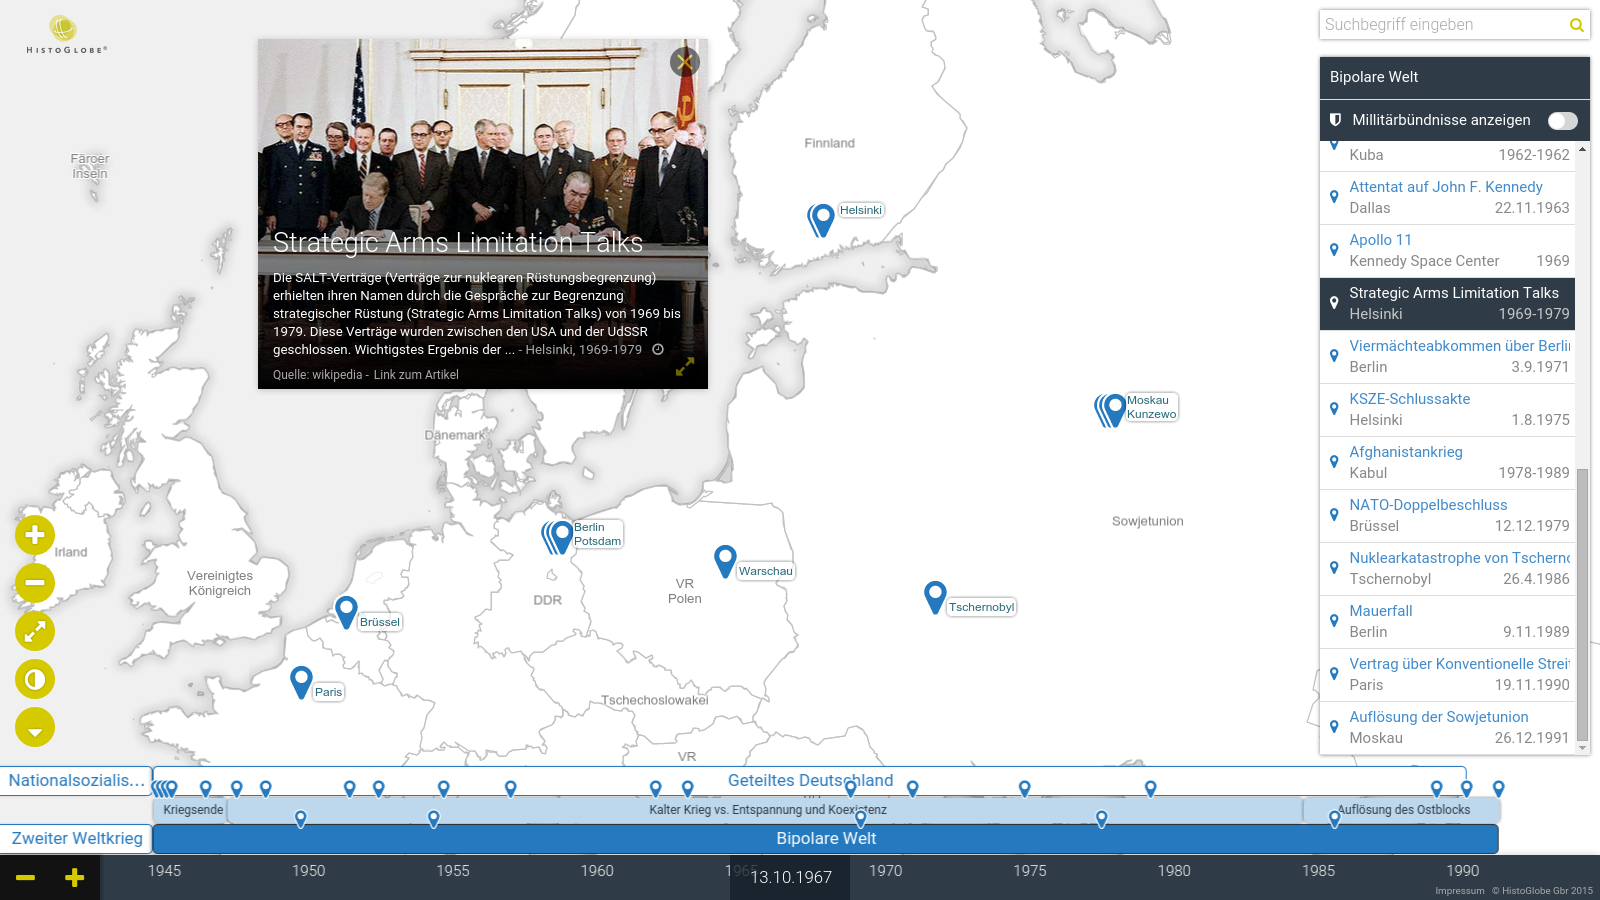
\includegraphics[width=0.9\textwidth]{graphics/final_ui.png}
  \caption{Hivent List}
\end{figure}

\subsubsection{Structure} % (fold)
\label{ssub:structure_hl}
The Hivent List module consists of title bar, an optional area and a list of hivents. The title bar and the optional area have a fixed size and a fixed distance to the search bar. The list has a fixed distance to the timeline and has the remaining amount available. 
Aufbau: Titel, Options, List


\subsubsection{Behaviour} % (fold)
\label{ssub:behaviour_hl}
Special Functionality: Knopp
Clickbar, Hoverbar
Slide into view on active
On Search only Headline is shown
dynamicly adapt to window heigth

% subsection hivent_list (end)
